\documentclass{standalone}
\usepackage{tikz}
\usetikzlibrary{patterns, positioning}
\usepackage[sfdefault]{ClearSans} %% option 'sfdefault' activates Clear Sans as the default text font
\usepackage[T1]{fontenc}

\begin{document}
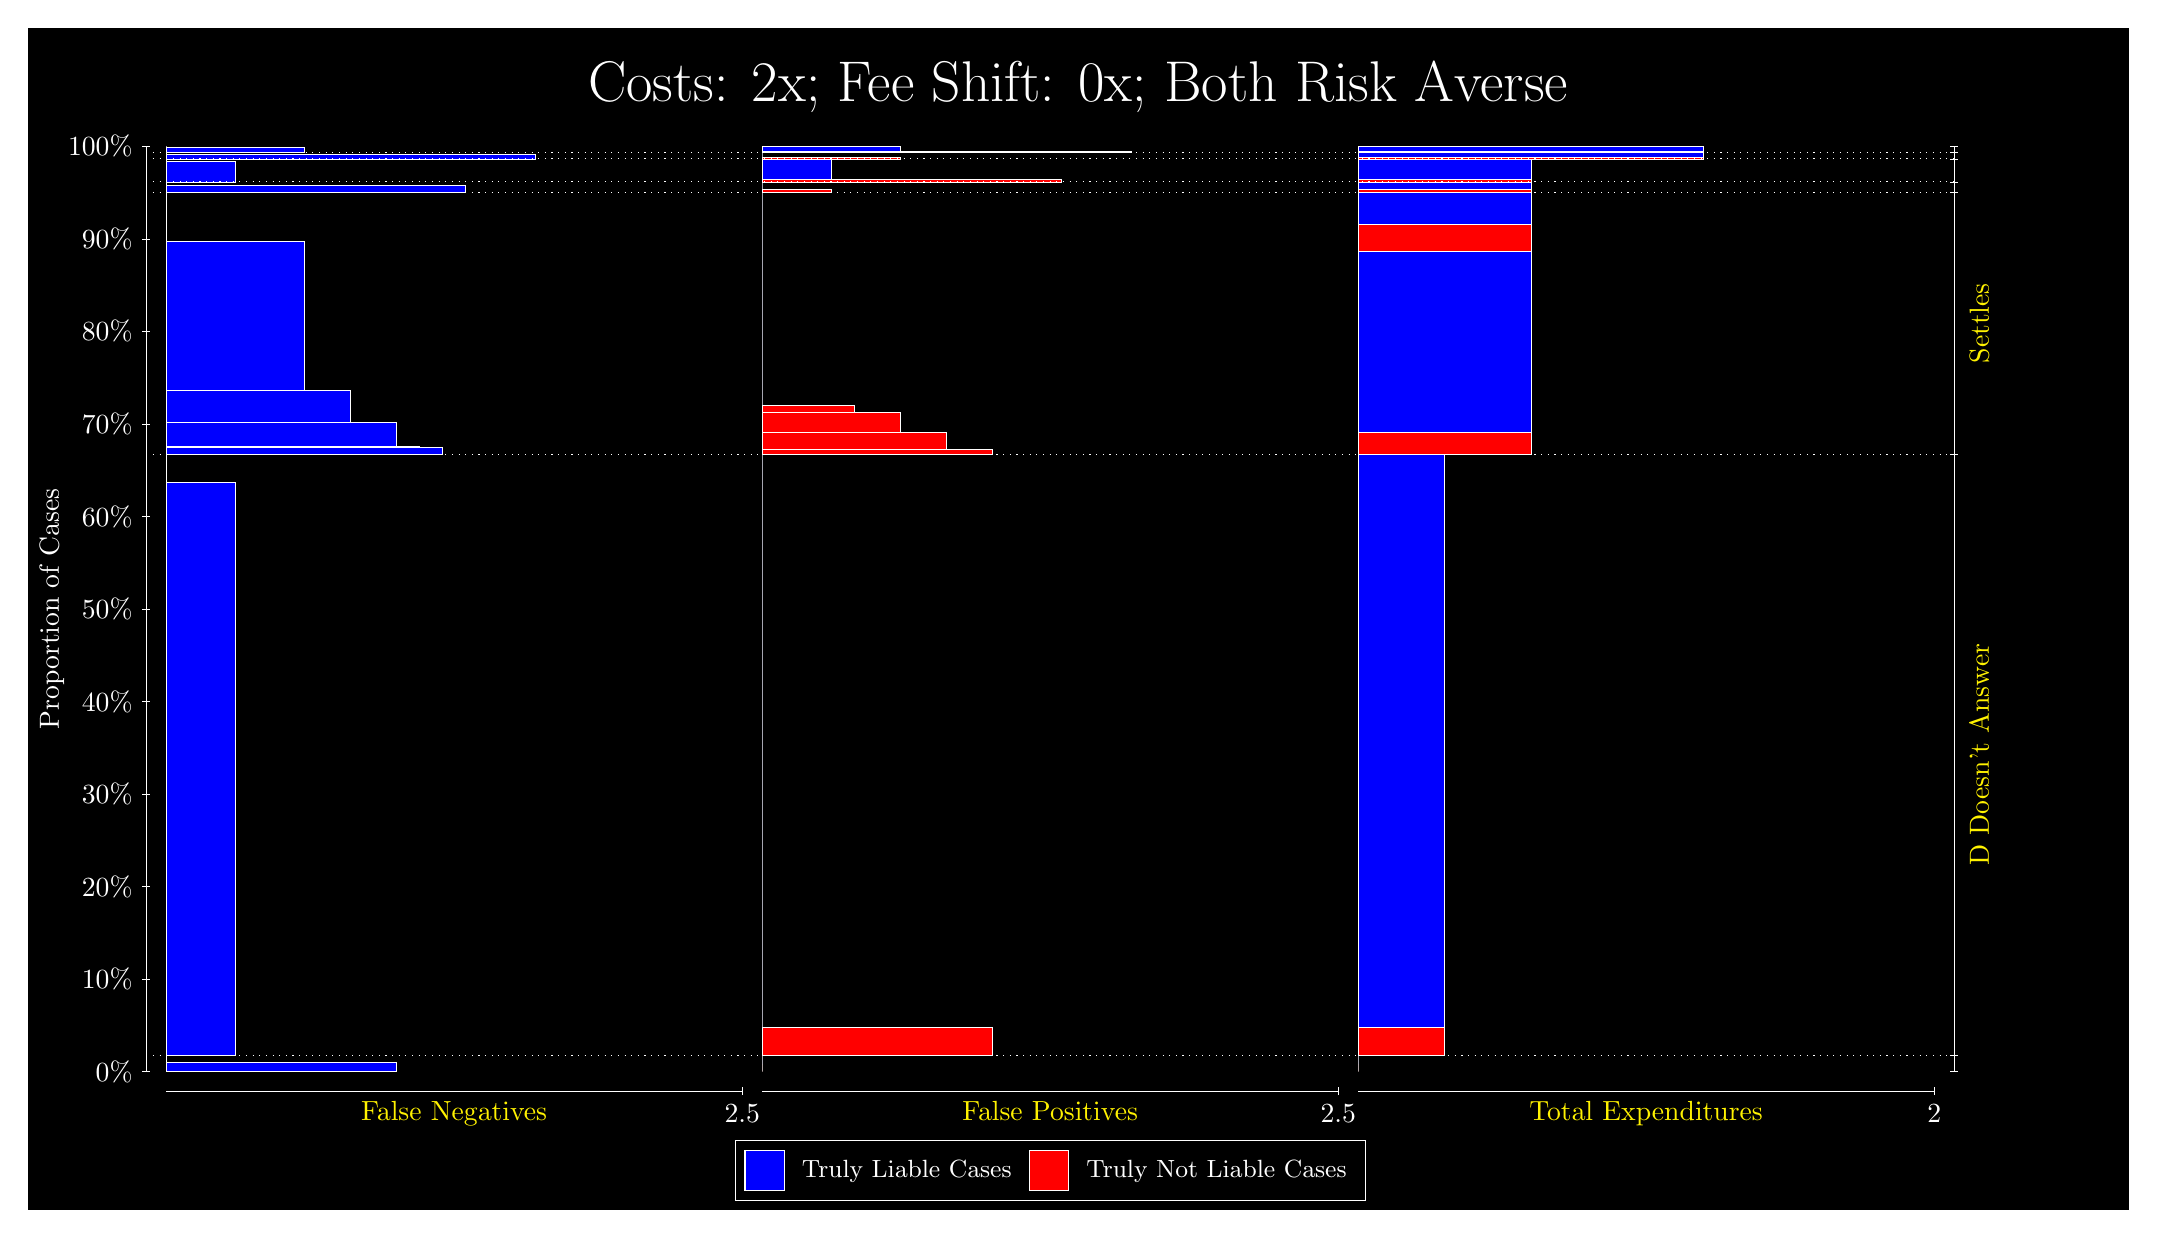
\begin{tikzpicture}
\draw[fill=black] (0,0) rectangle (26.667,15);
\draw[text=white] (0,13.5) rectangle (26.667,15) node[midway] {\huge Costs: 2x; Fee Shift: 0x; Both Risk Averse};
\draw[white, very thin] (1.5,1.75) -- (1.5,13.5);
\node[rotate=90, text=white, anchor=center] at (0.3, 7.625) {Proportion of Cases};
\draw[white, very thin] (1.45,1.75) -- (1.55,1.75);
\node[text=white, anchor=east] at (1.45, 1.75) {0\%};
\draw[white, very thin] (1.45,2.925) -- (1.55,2.925);
\node[text=white, anchor=east] at (1.45, 2.925) {10\%};
\draw[white, very thin] (1.45,4.1) -- (1.55,4.1);
\node[text=white, anchor=east] at (1.45, 4.1) {20\%};
\draw[white, very thin] (1.45,5.275) -- (1.55,5.275);
\node[text=white, anchor=east] at (1.45, 5.275) {30\%};
\draw[white, very thin] (1.45,6.45) -- (1.55,6.45);
\node[text=white, anchor=east] at (1.45, 6.45) {40\%};
\draw[white, very thin] (1.45,7.625) -- (1.55,7.625);
\node[text=white, anchor=east] at (1.45, 7.625) {50\%};
\draw[white, very thin] (1.45,8.8) -- (1.55,8.8);
\node[text=white, anchor=east] at (1.45, 8.8) {60\%};
\draw[white, very thin] (1.45,9.975) -- (1.55,9.975);
\node[text=white, anchor=east] at (1.45, 9.975) {70\%};
\draw[white, very thin] (1.45,11.15) -- (1.55,11.15);
\node[text=white, anchor=east] at (1.45, 11.15) {80\%};
\draw[white, very thin] (1.45,12.325) -- (1.55,12.325);
\node[text=white, anchor=east] at (1.45, 12.325) {90\%};
\draw[white, very thin] (1.45,13.5) -- (1.55,13.5);
\node[text=white, anchor=east] at (1.45, 13.5) {100\%};

\draw[white, very thin] (24.457,1.75) -- (24.457,13.5);
\draw[white, very thin] (24.407,1.75) -- (24.507,1.75);
\node[anchor=west] at (24.407, 1.75) {};
\draw[white, very thin] (24.407,1.9584) -- (24.507,1.9584);
\node[anchor=west] at (24.407, 1.9584) {};
\draw[white, very thin] (24.407,9.5891) -- (24.507,9.5891);
\node[anchor=west] at (24.407, 9.5891) {};
\draw[white, very thin] (24.407,12.918) -- (24.507,12.918);
\node[anchor=west] at (24.407, 12.918) {};
\draw[white, very thin] (24.407,13.049) -- (24.507,13.049);
\node[anchor=west] at (24.407, 13.049) {};
\draw[white, very thin] (24.407,13.34) -- (24.507,13.34);
\node[anchor=west] at (24.407, 13.34) {};
\draw[white, very thin] (24.407,13.424) -- (24.507,13.424);
\node[anchor=west] at (24.407, 13.424) {};
\draw[white, very thin] (24.407,13.5) -- (24.507,13.5);
\node[anchor=west] at (24.407, 13.5) {};

\draw[white, very thin, fill=blue] (1.75,1.75) rectangle (4.6775,1.8649);
\draw[white, very thin, fill=red] (1.75,1.8649) rectangle (1.75,1.9584);
\draw[white, very thin, fill=blue] (1.75,1.9584) rectangle (2.6283,9.2359);
\draw[white, very thin, fill=red] (1.75,9.2359) rectangle (1.75,9.5891);
\draw[white, very thin, fill=blue] (1.75,9.5891) rectangle (5.2631,9.6841);
\draw[white, very thin, fill=blue] (1.75,9.6841) rectangle (4.9703,9.6901);
\draw[white, very thin, fill=blue] (1.75,9.6901) rectangle (4.6775,9.996);
\draw[white, very thin, fill=blue] (1.75,9.996) rectangle (4.092,10.398);
\draw[white, very thin, fill=blue] (1.75,10.398) rectangle (3.5065,12.292);
\draw[white, very thin, fill=red] (1.75,12.292) rectangle (1.75,12.918);
\draw[white, very thin, fill=blue] (1.75,12.918) rectangle (5.5558,13.009);
\draw[white, very thin, fill=red] (1.75,13.009) rectangle (1.75,13.049);
\draw[white, very thin, fill=blue] (1.75,13.049) rectangle (2.6283,13.308);
\draw[white, very thin, fill=red] (1.75,13.308) rectangle (1.75,13.34);
\draw[white, very thin, fill=blue] (1.75,13.34) rectangle (6.4341,13.401);
\draw[white, very thin, fill=red] (1.75,13.401) rectangle (1.75,13.424);
\draw[white, very thin, fill=blue] (1.75,13.424) rectangle (3.5065,13.493);
\draw[white, very thin, fill=red] (1.75,13.493) rectangle (1.75,13.5);
\draw[white, very thin, fill=red] (9.3189,1.75) rectangle (9.3189,1.8435);
\draw[white, very thin, fill=blue] (9.3189,1.8435) rectangle (9.3189,1.9584);
\draw[white, very thin, fill=red] (9.3189,1.9584) rectangle (12.246,2.3117);
\draw[white, very thin, fill=blue] (9.3189,2.3117) rectangle (9.3189,9.5891);
\draw[white, very thin, fill=red] (9.3189,9.5891) rectangle (12.246,9.6573);
\draw[white, very thin, fill=red] (9.3189,9.6573) rectangle (11.661,9.8726);
\draw[white, very thin, fill=red] (9.3189,9.8726) rectangle (11.075,10.123);
\draw[white, very thin, fill=red] (9.3189,10.123) rectangle (10.783,10.127);
\draw[white, very thin, fill=red] (9.3189,10.127) rectangle (10.49,10.215);
\draw[white, very thin, fill=blue] (9.3189,10.215) rectangle (9.3189,12.918);
\draw[white, very thin, fill=red] (9.3189,12.918) rectangle (10.197,12.958);
\draw[white, very thin, fill=blue] (9.3189,12.958) rectangle (9.3189,13.049);
\draw[white, very thin, fill=red] (9.3189,13.049) rectangle (13.125,13.081);
\draw[white, very thin, fill=blue] (9.3189,13.081) rectangle (10.197,13.34);
\draw[white, very thin, fill=red] (9.3189,13.34) rectangle (11.075,13.364);
\draw[white, very thin, fill=blue] (9.3189,13.364) rectangle (9.3189,13.424);
\draw[white, very thin, fill=red] (9.3189,13.424) rectangle (14.003,13.431);
\draw[white, very thin, fill=blue] (9.3189,13.431) rectangle (11.075,13.5);
\draw[white, very thin, fill=red] (16.888,1.75) rectangle (16.888,1.8435);
\draw[white, very thin, fill=blue] (16.888,1.8435) rectangle (16.888,1.9584);
\draw[white, very thin, fill=red] (16.888,1.9584) rectangle (17.986,2.3117);
\draw[white, very thin, fill=blue] (16.888,2.3117) rectangle (17.986,9.5891);
\draw[white, very thin, fill=red] (16.888,9.5891) rectangle (19.083,9.8726);
\draw[white, very thin, fill=blue] (16.888,9.8726) rectangle (19.083,12.169);
\draw[white, very thin, fill=red] (16.888,12.169) rectangle (19.083,12.512);
\draw[white, very thin, fill=blue] (16.888,12.512) rectangle (19.083,12.918);
\draw[white, very thin, fill=red] (16.888,12.918) rectangle (19.083,12.958);
\draw[white, very thin, fill=blue] (16.888,12.958) rectangle (19.083,13.049);
\draw[white, very thin, fill=red] (16.888,13.049) rectangle (19.083,13.081);
\draw[white, very thin, fill=blue] (16.888,13.081) rectangle (19.083,13.34);
\draw[white, very thin, fill=red] (16.888,13.34) rectangle (21.279,13.364);
\draw[white, very thin, fill=blue] (16.888,13.364) rectangle (21.279,13.424);
\draw[white, very thin, fill=red] (16.888,13.424) rectangle (21.279,13.431);
\draw[white, very thin, fill=blue] (16.888,13.431) rectangle (21.279,13.5);
\draw[white, dotted] (1.5,1.9584) -- (24.457,1.9584);
\draw[white, dotted] (1.5,9.5891) -- (24.457,9.5891);
\draw[white, dotted] (1.5,12.918) -- (24.457,12.918);
\draw[white, dotted] (1.5,13.049) -- (24.457,13.049);
\draw[white, dotted] (1.5,13.34) -- (24.457,13.34);
\draw[white, dotted] (1.5,13.424) -- (24.457,13.424);
\draw[white, very thin] (1.75,1.5) -- (9.0689,1.5);
\node[text=yellow, anchor=north] at (5.4094, 1.5) {False Negatives};
\draw[white, very thin] (9.0689,1.45) -- (9.0689,1.55);
\node[text=white, anchor=north] at (9.0689, 1.45) {2.5};

\draw[white, very thin] (9.3189,1.5) -- (16.638,1.5);
\node[text=yellow, anchor=north] at (12.978, 1.5) {False Positives};
\draw[white, very thin] (16.638,1.45) -- (16.638,1.55);
\node[text=white, anchor=north] at (16.638, 1.45) {2.5};

\draw[white, very thin] (16.888,1.5) -- (24.207,1.5);
\node[text=yellow, anchor=north] at (20.547, 1.5) {Total Expenditures};
\draw[white, very thin] (24.207,1.45) -- (24.207,1.55);
\node[text=white, anchor=north] at (24.207, 1.45) {2};


\node[text=yellow, centered, rotate=90] at (24.777, 5.7738) {D Doesn't Answer};
\node[text=yellow, centered, rotate=90] at (24.777, 11.254) {Settles};





\draw (12.978300999999998,1.5) node[draw=none] (baseCoordinate) {};
\begin{scope}[align=center]
        \matrix[scale=0.5, draw=white, below=0.5cm of baseCoordinate, nodes={draw}, column sep=0.1cm]{
            \node[rectangle, draw, minimum width=0.5cm, minimum height=0.5cm, fill=blue] {}; &
            \node[draw=none, font=\small, text=white] (B) {Truly Liable Cases}; &
            \node[rectangle, draw, minimum width=0.5cm, minimum height=0.5cm, fill=red] {}; &
            \node[draw=none, font=\small, text=white] (B) {Truly Not Liable Cases}; \\
            };
\end{scope}

\end{tikzpicture}
\end{document}